\documentclass[12pt,a4paper]{article}

\usepackage[utf8]{inputenc}
\usepackage[T1]{fontenc}
\usepackage[spanish,es-tabla]{babel}
\usepackage{mathpazo}
\usepackage{microtype}
\usepackage{setspace}
\usepackage[a4paper,margin=2.5cm,headheight=14pt]{geometry}
\usepackage{fancyhdr}
\usepackage{amsmath,amssymb}
\usepackage{graphicx}
\usepackage{booktabs}
\usepackage{array}
\usepackage{xcolor}
\usepackage{caption}
\usepackage{float}
\usepackage{tikz}
\usetikzlibrary{arrows.meta,positioning}
\usepackage{hyperref}

\definecolor{arena}{HTML}{8C2F1B}

\hypersetup{
  colorlinks=true,
  linkcolor=arena,
  citecolor=arena,
  urlcolor=arena,
  pdftitle={Arena FPS: informe de desarrollo},
  pdfauthor={Simón Díaz Monroy}
}

\setstretch{1.15}
\setlength{\parindent}{1.2em}
\setlength{\parskip}{0.2em}
\setlength{\emergencystretch}{2em}

\pagestyle{fancy}
\fancyhf{}
\fancyhead[L]{\small Arena FPS}
\fancyhead[R]{\small Informe de desarrollo}
\fancyfoot[C]{\thepage}
\renewcommand{\headrulewidth}{0.4pt}

\captionsetup{font=small,labelfont=bf}
\graphicspath{{diagrams/}{../presentation/img/}}

\begin{document}
\shorthandoff{<>}

% ---------------------------------------------------------------------------
% Portada
% ---------------------------------------------------------------------------
\hypersetup{pageanchor=false}
\begin{titlepage}
  \centering
  \vspace*{1.8cm}
  {\large Computación Gráfica\par}
  \vspace{1.6cm}
  {\Huge\bfseries Arena FPS\par}
  \vspace{0.5cm}
  {\LARGE Motor de disparos en primera persona\\[0.2cm] sobre OpenGL 3.3\par}
  \vspace{1.6cm}
  {\large Informe de desarrollo\par}
  \vfill
  {\large Simón Díaz Monroy\par}
  \vspace{0.3cm}
  {\large \today\par}
  \vspace{1.2cm}
  \rule{0.55\textwidth}{0.4pt}
\end{titlepage}
\hypersetup{pageanchor=true}

% ---------------------------------------------------------------------------
% Resumen
% ---------------------------------------------------------------------------
\section*{Resumen}

Arena FPS es un motor de disparos en primera persona construido sobre OpenGL
3.3 \emph{core}. El proyecto integra carga de geometría, colisión, movimiento,
combate y lectura de niveles sin bibliotecas de física externas. El resultado es
una arena con dos niveles, tres tipos de enemigo, un arma de impacto
instantáneo, llaves, puertas, trampas y salidas. Este informe resume las
decisiones principales y el estado real de la implementación.

\vspace{0.4em}
\noindent\textbf{Palabras clave:} motor de juego, OpenGL, colisiones AABB,
movimiento estilo Quake, formato de nivel.

% ---------------------------------------------------------------------------
\section{Introducción}
% ---------------------------------------------------------------------------

Arena FPS se construyó como un ejercicio de motor pequeño. La meta fue reunir en
un mismo proyecto la carga de mallas, el trazado de rayos, la simulación del
jugador, el combate y la lectura de niveles, usando OpenGL como única interfaz de
renderización. La escala reducida permitió tomar decisiones que en un motor
general serían discutibles: colisión limitada a cajas alineadas con los ejes,
personajes dibujados con cubos, texturas sustituidas por colores y movimiento
basado en las reglas de Quake. Ninguna de esas simplificaciones es accidental;
todas reducen los sistemas que deben convivir.
% ---------------------------------------------------------------------------
\section{Restricciones y alcance}
% ---------------------------------------------------------------------------

Los gráficos se implementan únicamente con OpenGL: GLFW gestiona la ventana y la
entrada, GLAD carga las funciones y GLM aporta el álgebra lineal, pero la
secuencia de dibujo, los sombreadores y las mallas son responsabilidad del
proyecto. Tampoco se emplean bibliotecas de física externas: la gravedad, la
fricción, la aceleración, el salto, las colisiones y el trazado de rayos se
escribieron a mano.

El alcance deja fuera el sonido, las animaciones y las texturas. Los personajes
y objetos se representan con sólidos platónicos; en la versión actual, con
cubos. El
diseño de niveles se limita a dos mapas y a un recorrido cerrado: encontrar la
llave, sobrevivir a la emboscada, abrir la puerta y llegar a la salida.

% ---------------------------------------------------------------------------
\section{Arquitectura general}
% ---------------------------------------------------------------------------

El código se organiza en módulos con dependencias en una sola dirección
(figura~\ref{fig:paquetes}). \texttt{main} conoce la ventana, el contexto de
OpenGL, la entrada y el bucle; \texttt{game} contiene el estado y las reglas;
\texttt{physics} resuelve cuerpos y colisiones; \texttt{level} carga geometría y
datos; \texttt{render} dibuja la escena; \texttt{ui} integra Dear ImGui; y
\texttt{gl} agrupa cámara, mallas y sombreadores.

\begin{figure}[htbp]
  \centering
  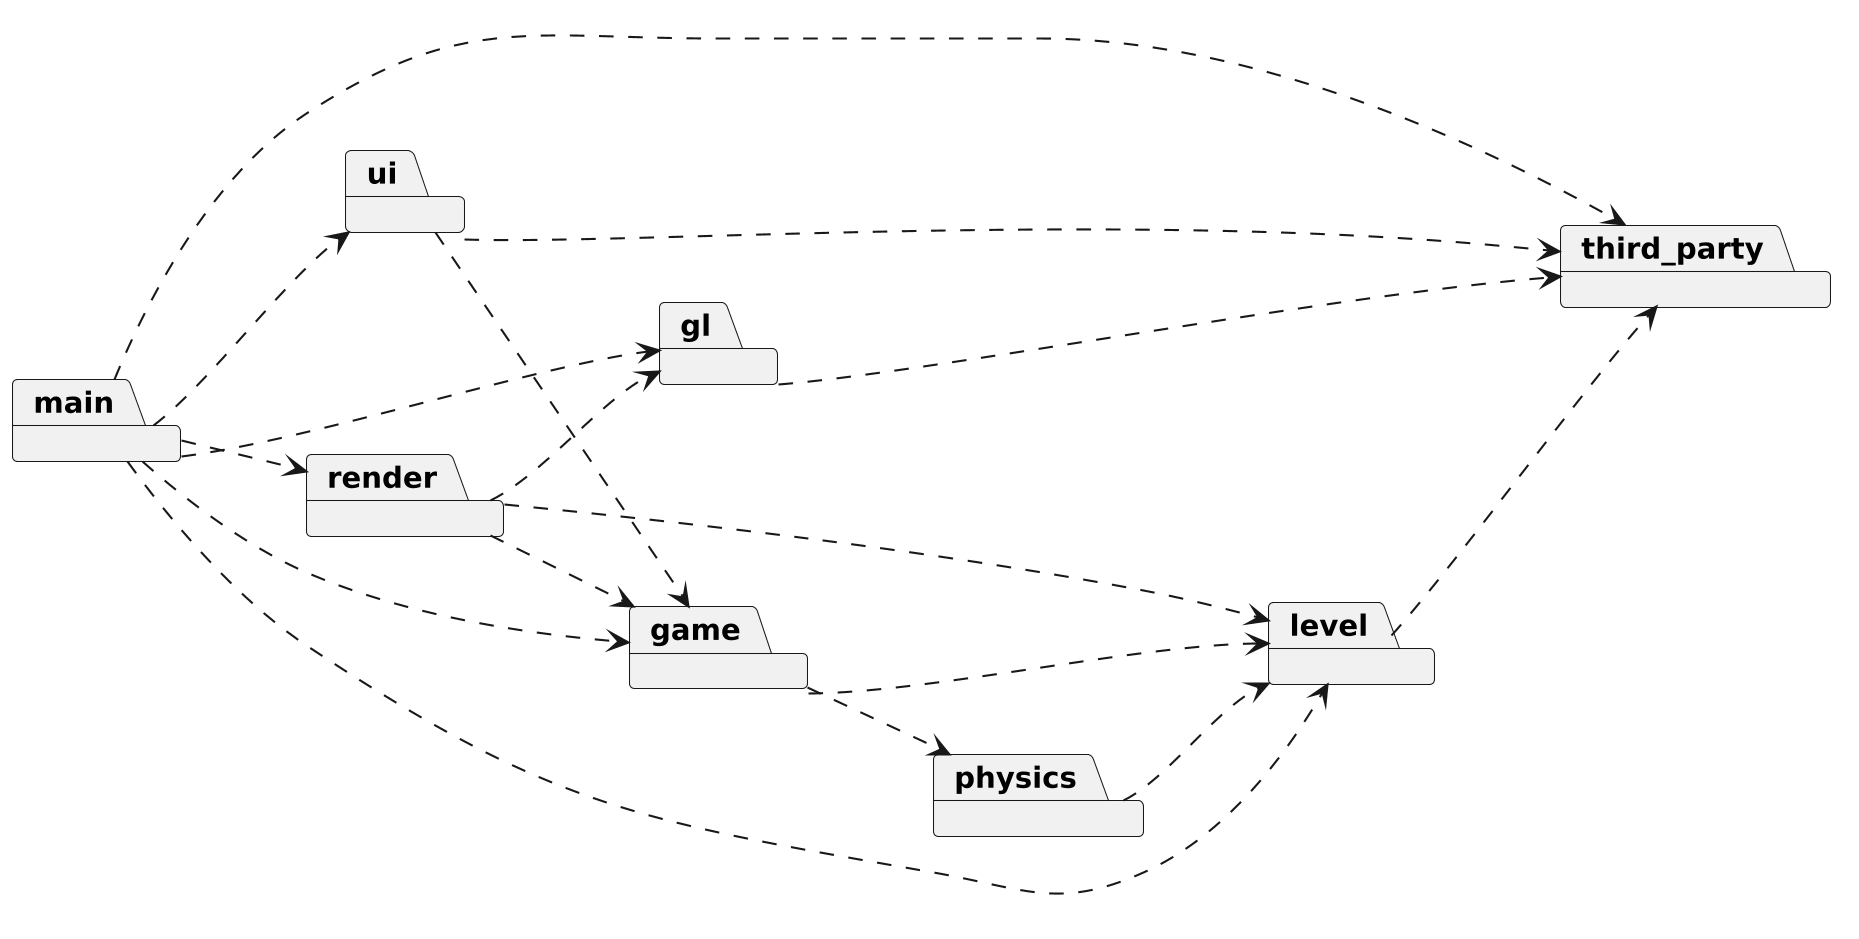
\includegraphics[width=0.88\textwidth]{packages.png}
  \caption{Organización de paquetes y dependencias principales.}
  \label{fig:paquetes}
\end{figure}

La separación se apoya en una regla: \texttt{World} no incluye cabeceras de
OpenGL y \texttt{SceneRenderer} recibe el mundo como referencia constante. El
primero puede ejecutarse sin contexto gráfico; el segundo no puede modificar la
partida. \texttt{Level} permanece inmutable durante el juego y
\texttt{World::Initialize} copia su estado inicial, de modo que reiniciar no
exige volver a leer archivos.

El bucle acumula tiempo real y ejecuta pasos constantes de $1/120$~s mientras el
acumulador alcance. Así la física no depende de la tasa de fotogramas. El tiempo
de fotograma se limita a $0.25$~s para evitar ráfagas de actualizaciones tras
una pausa larga.

% ---------------------------------------------------------------------------
\section{Física}
% ---------------------------------------------------------------------------

\subsection{Colisión y trazado de rayos}

El jugador y los enemigos son cuerpos rectangulares definidos por un centro,
unas semiextensiones y una velocidad; su colisión usa cajas delimitadoras
alineadas con los ejes (AABB). La caja que ocupan se obtiene restando y sumando
las semiextensiones al centro. El mundo de colisión se construye a
partir de los volúmenes del nivel y solo cambia cuando una puerta se abre y
desactiva su colisionador. El solapamiento es estricto: dos cajas se cruzan
únicamente si sus intervalos se superponen en los tres ejes, de modo que tocar
una cara sin penetrar no cuenta \cite{mdn}.

El desplazamiento se resuelve por ejes: primero $x$, después $z$ y por último
$y$. En cada eje, si hay solapamiento, la posición se ajusta a la cara del
volumen y se anula la componente de velocidad correspondiente. El orden
horizontal antes que el vertical evita que una pared detectada tarde arrastre al
cuerpo hacia arriba o hacia abajo. La resolución genera contactos con índice de
volumen, normal y profundidad; la política de movimiento usa los indicadores de
suelo, techo y pared.

El trazado de rayos emplea la prueba de losas. Para cada eje se calculan las
distancias paramétricas de entrada y salida de la caja, se ordenan y se conserva
la mayor entrada y la menor salida:

\[
  t_{\min}=\max(t_1,t_2,t_3),\qquad
  t_{\max}=\min(t_4,t_5,t_6).
\]

Hay impacto si $t_{\min}\le t_{\max}$ y $t_{\max}\ge 0$. La normal se obtiene
del eje que produjo la entrada; si el origen ya está dentro de la caja, se
devuelve la dirección opuesta al rayo. La misma consulta se utiliza para el arma y
para la línea de visión de los enemigos.

\subsection{Gravedad, aceleración y fricción}

La gravedad es de $-20$~m/s$^2$; la velocidad vertical se limita a $50$~m/s y el
salto parte de $6.9$~m/s, lo que produce una altura máxima cercana a $1.19$~m.
La aceleración en el suelo proyecta la velocidad sobre la dirección deseada
$\hat{w}$ y añade un incremento limitado por la velocidad objetivo:
\[
  v_p=\vec{v}\cdot\hat{w},\qquad
  \Delta v=\min\left(a\,v_{\text{obj}}\Delta t,\;v_{\text{obj}}-v_p\right).
\]
La fricción se aplica antes de acelerar y reduce la velocidad horizontal de
forma lineal, con una velocidad de parada que evita el deslizamiento perpetuo:
\[
  v'=\max\left(0,\;v-\max(v,v_{\text{parada}})\,f\,\Delta t\right).
\]
En el aire se limita la velocidad objetivo a $0.8$~m/s antes de calcular la
diferencia, aunque el incremento se calcula con la velocidad objetivo original.
Esa asimetría permite ganar velocidad al girar y desplazarse de lado.

La fuerza de empuje está prevista para impactos de enemigos y explosiones, pero
no interviene todavía porque no hay proyectiles explosivos.

% ---------------------------------------------------------------------------
\section{Movimiento}
% ---------------------------------------------------------------------------

La cámara es de primera persona: el ratón cambia la orientación, el botón
izquierdo dispara y las teclas W, A, S y D desplazan al jugador. La barra
espaciadora salta; Escape libera el cursor y un clic posterior lo recaptura. F1
muestra las cajas de colisión, F2 alterna el salto automático, F3 activa el
movimiento libre y R reinicia tras una muerte.

El controlador reproduce las reglas de Quake \cite{quake}: fricción y
aceleración en el suelo, aceleración distinta en el aire y salto con impulso. La
literatura sobre el salto de conejo (\emph{bunny hopping}) y el salto lateral
(\emph{strafe jumping}) \cite{adrian,tuni,matt} explica que la ganancia de
velocidad no proviene de una fuerza adicional, sino de la proyección favorable
de la velocidad sobre la dirección deseada en cada paso. El encadenamiento de
saltos conserva el impulso; el modo automático de F2 repite el salto mientras la
tecla esté pulsada. El salto con cohete queda pendiente porque requiere
explosiones con fuerza de empuje.

% ---------------------------------------------------------------------------
\section{Combate}
% ---------------------------------------------------------------------------

El arma implementada es de impacto instantáneo (\emph{hitscan}). Al disparar se
lanza un rayo desde la cámara, se busca el enemigo vivo más cercano y se compara
su distancia con la del primer volumen del nivel. Si el enemigo está antes que
la pared, recibe $25$ puntos de daño; el alcance es de $40$~m y la cadencia de
$0.15$~s. El misil sería un proyectil lento y visible; la granada, un proyectil
explosivo con empuje. Ninguna de las dos armas está implementada: ambas
exigirían cuerpos móviles, integración y colisión propia.

La tabla~\ref{tab:enemigos} recoge los parámetros de los tres enemigos. Su
comportamiento es una máquina de estados con patrulla, persecución y ataque
(figura~\ref{fig:fsm}). La visión se comprueba con un rayo desde los ojos del
enemigo hasta el jugador. El movimiento es en línea recta y la colisión impide
atravesar paredes; no hay cálculo de rutas.

\begin{table}[htbp]
  \centering
  \small
  \begin{tabular}{@{}lrrrrrr@{}}
    \toprule
    Tipo & Velocidad & Visión & Alcance & Intervalo & Salud & Daño \\
         & (m/s) & (m) & (m) & (s) & & \\
    \midrule
    Cuerpo a cuerpo & 6.0 & 35 & 1.2 & 0.8 & 50 & 10 \\
    A distancia     & 4.5 & 45 & 15.0 & 1.5 & 30 & 8 \\
    Tanque          & 1.8 & 35 & 20.0 & 2.0 & 120 & 15 \\
    \bottomrule
  \end{tabular}
  \caption{Parámetros de los tres tipos de enemigo.}
  \label{tab:enemigos}
\end{table}

\begin{figure}[htbp]
  \centering
  \begin{tikzpicture}[
      ->, >=Latex, shorten >=2pt, node distance=2.5cm,
      state/.style={draw, rounded corners, fill=arena!8, minimum width=2.3cm,
                    minimum height=0.8cm, font=\small},
      auto, font=\scriptsize
    ]
    \node[state] (p) {Patrulla};
    \node[state, right=of p] (c) {Persecución};
    \node[state, below=of c] (a) {Ataque};
    \draw (p) edge[bend left] node[above] {ve al jugador} (c);
    \draw (c) edge[bend left] node[below] {pierde de vista} (p);
    \draw (c) edge[bend left] node[right] {en alcance} (a);
    \draw (a) edge[bend left] node[left] {fuera de alcance} (c);
  \end{tikzpicture}
  \caption{Máquina de estados del enemigo.}
  \label{fig:fsm}
\end{figure}

% ---------------------------------------------------------------------------
\section{Niveles y mapas}
% ---------------------------------------------------------------------------

El primer nivel es introductorio: una sala, un pasillo, una llave, una puerta y
una salida al segundo nivel. Los enemigos de cuerpo a cuerpo patrullan la sala y
los de distancia custodian la salida tras la puerta. El segundo nivel es el mapa
de trampas: la llave está protegida por un tanque y dos enemigos a distancia, el
pasillo causa daño constante y la sala final tiene una franja dañina y tres
salidas. Una vuelve al nivel uno, otra reinicia el nivel dos y la tercera solo
completa la partida.

Cada nivel se divide en un archivo \texttt{.obj} con la geometría visible y un
archivo \texttt{.lvl} con el comportamiento, una instrucción por línea. El
analizador es propio y no añade dependencias; el formato se definió antes de
construir el primer nivel. La tabla~\ref{tab:lvl} recoge las instrucciones. Los valores se separan por espacios
y \texttt{\#} inicia un comentario.

\begin{table}[htbp]
  \centering
  \footnotesize
  \begin{tabular}{@{}>{\raggedright\arraybackslash}p{0.49\textwidth}>{\raggedright\arraybackslash}p{0.43\textwidth}@{}}
    \toprule
    Instrucción & Significado \\
    \midrule
    \texttt{player x y z} & Posición inicial del jugador. \\
    \texttt{brush minX minY minZ maxX maxY maxZ} &
      Caja de colisión y superficie por defecto. \\
    \texttt{door brushIndex keyId} &
      Puerta que se abre al tocarla con la llave \texttt{keyId}. \\
    \texttt{key keyId x y z} & Llave recogible. \\
    \texttt{exit minX minY minZ maxX maxY maxZ [nextLevel]} &
      Volumen no sólido que completa el nivel y, si se indica, carga
      \texttt{nextLevel}. \\
    \texttt{light x y z r g b intensity} & Luz puntual. \\
    \texttt{enemy type x y z [x2 y2 z2]} &
      Enemigo; con el segundo trío, patrulla entre ambos puntos. \\
    \texttt{trap brushIndex damagePerSecond} &
      Superficie que causa daño por segundo. \\
    \bottomrule
  \end{tabular}
  \caption{Instrucciones del archivo \texttt{.lvl}.}
  \label{tab:lvl}
\end{table}

Los volúmenes se numeran en orden de aparición y \texttt{door} y \texttt{trap}
los referencian por índice. La carga del nivel impone las siguientes reglas:

\begin{enumerate}
  \item Todo volumen no marcado como trampa es suelo.
  \item Un volumen no puede ser puerta y trampa a la vez.
  \item Los identificadores de llave son únicos: una puerta puede compartir
        llave con otras, pero no apuntar a una inexistente.
  \item Las llaves se consumen al recogerse y la puerta queda abierta de forma
        permanente.
  \item La salida nunca bloquea el movimiento.
\end{enumerate}

La salida exige una instrucción \texttt{player} y al menos una salida; se aplica
la primera que se toca. Las coordenadas mínimas no pueden superar a las máximas
y los errores se informan con archivo y línea, sin modificar el nivel ya
cargado.

La geometría visible se modela en Blender y se exporta a \texttt{.obj}; el
trazado de salas y alturas siguió las recomendaciones generales de diseño de
mapas \cite{map}. La colisión se declara aparte con volúmenes, lo que permite
tener detalle visual sin encarecer la simulación.

% ---------------------------------------------------------------------------
\section{Diseño visual}
% ---------------------------------------------------------------------------

La dirección visual reduce los personajes a sólidos platónicos y prescinde de
animaciones. El cubo unitario se reutiliza para enemigos, llaves, puertas,
trampas y salida, con traslación y escala. Las texturas y materiales se
sustituyen por colores planos que identifican el tipo de enemigo, su estado y
los objetos interactivos.

La iluminación se resuelve en el sombreador de fragmentos con una luz puntual.
El color combina un ambiente del $20$\,\% con una difusa atenuada por
$1/(1+0.02d^2)$. El nivel es una cáscara cerrada vista desde dentro; como las
normales exportadas apuntan hacia fuera, el sombreador las invierte en las caras
traseras. El renderizador usa solo la primera instrucción \texttt{light} del
nivel y, si no hay ninguna, aplica una luz de relleno. La salida se dibuja como
una caja verde translúcida y la depuración de colisión, activada con F1, muestra
los volúmenes en malla de alambre. La interfaz presenta salud, velocidad y mira.

El sonido quedó fuera del alcance: no hay subsistema de audio, carga de archivos
ni mezcla.

% ---------------------------------------------------------------------------
\section{Herramientas y dependencias}
% ---------------------------------------------------------------------------

\begin{table}[htbp]
  \centering
  \small
  \begin{tabular}{@{}ll@{}}
    \toprule
    Área & Decisión \\
    \midrule
    Ventana y entrada & GLFW 3.4 \\
    OpenGL & 3.3 \emph{core} \\
    Carga de funciones & GLAD (OpenGL 3.3 \emph{core}, perfil \emph{core}) \\
    Matemáticas & GLM 1.0.1 \\
    Construcción & CMake $\geq$ 3.16, C++20 \\
    Geometría de mapas & tinyobjloader 1.0.6 \\
    Interfaz de usuario & Dear ImGui \\
    \bottomrule
  \end{tabular}
  \caption{Herramientas y dependencias principales.}
  \label{tab:herramientas}
\end{table}

GLM aporta vectores, matrices y proyecciones. GLAD se generó con \texttt{glad2}
para OpenGL 3.3 \emph{core}. tinyobjloader carga la geometría \texttt{.obj}; es
de cabecera única y licencia MIT. Dear ImGui se usa para la interfaz y los
paneles de depuración.

Se prefirió GLFW sobre GLUT porque Dear ImGui ofrece una integración estable con
GLFW y porque GLUT está en desuso. OpenGL y GLFW se enlazan contra las
bibliotecas del sistema; GLM, GLAD y tinyobjloader se incluyen en
\texttt{src/third\_party}. La construcción usa CMake y el ejecutable se llama
\texttt{arena}.

% ---------------------------------------------------------------------------
\section{Estado de implementación}
% ---------------------------------------------------------------------------

\begin{table}[H]
  \centering
  \footnotesize
  \renewcommand{\arraystretch}{1.05}
  \begin{tabular}{@{}>{\raggedright\arraybackslash}p{0.32\textwidth}>{\raggedright\arraybackslash}p{0.14\textwidth}>{\raggedright\arraybackslash}p{0.46\textwidth}@{}}
    \toprule
    Subsistema & Estado & Observaciones \\
    \midrule
    Núcleo & Completo &
      Ventana GLFW 3.4, OpenGL 3.3 \emph{core}, GLAD, entrada, captura de ratón
      y paso fijo de $1/120$~s. \\
    Movimiento y colisión & Completo &
      Fricción, aceleración terrestre y aérea, salto, salto automático,
      resolución AABB por ejes y trazado de rayos. \\
    Combate & Completo &
      Arma \emph{hitscan} ($25$ de daño, $40$~m, $0.15$~s) y tres enemigos con
      patrulla, persecución y ataque. \\
    Niveles & Completo &
      \texttt{.obj} con tinyobjloader, \texttt{.lvl} propio, llaves, puertas,
      trampas, salidas y cambio de nivel. \\
    Presentación & Completo &
      Malla, cubos, luz puntual, transparencia, depuración de colisión e
      interfaz con Dear ImGui. \\
    Proyectiles y empuje & Pendiente &
      Requieren cuerpos móviles, explosiones y respuesta física sobre el
      jugador. \\
    Menú y pausa & Pendiente &
      Solo existen \texttt{Playing} y \texttt{PlayerDead}. \\
    Animaciones, texturas y sonido & Fuera de alcance &
      La dirección visual usa colores planos y no hay audio. \\
    \bottomrule
  \end{tabular}
  \caption{Estado de implementación por subsistema.}
  \label{tab:estado}
\end{table}

La versión actual se puede recorrer de principio a fin: la llave abre la puerta,
los enemigos responden según su tipo, las trampas restan salud y la salida carga
el nivel siguiente. Las limitaciones visibles son la ausencia de proyectiles, la
falta de empuje por explosiones y la existencia de una sola luz puntual. Los
enemigos no calculan rutas y el menú o la pausa no están implementados.

% ---------------------------------------------------------------------------
\section{Consideraciones finales}
% ---------------------------------------------------------------------------

El desarrollo permitió comprobar que un conjunto pequeño de reglas bien
delimitadas basta para producir una experiencia de disparos reconocible. La
restricción de OpenGL obligó a escribir la carga de mallas, los sombreadores y
el estado de la GPU; la prohibición de bibliotecas de física obligó a justificar
cada constante del movimiento y cada paso de la resolución de colisiones. La
separación entre \texttt{Level}, \texttt{World} y \texttt{SceneRenderer} facilitó
el reinicio y el cambio de mapa sin mezclar reglas de juego con dibujo.

Quedan pendientes los proyectiles y las explosiones con empuje, la iluminación
con varias luces, una navegación de enemigos que rodee obstáculos y un menú de
pausa. Ninguna de esas ampliaciones exige romper la arquitectura actual; todas
encajan en los módulos existentes.

% ---------------------------------------------------------------------------
% Referencias
% ---------------------------------------------------------------------------
\begingroup
\sloppy
\raggedright
\begin{thebibliography}{9}
\small

\bibitem{mdn} Mozilla, ``3D collision detection,'' \emph{MDN Web Docs}.
[En línea]. Disponible en:
\url{https://developer.mozilla.org/en-US/docs/Games/Techniques/3D_collision_detection}.
[Consultado: 25 nov. 2026].

\bibitem{quake} id Software, ``sv\_user.c,'' \emph{Quake source code}, GitHub.
[En línea]. Disponible en:
\url{https://github.com/id-Software/Quake/blob/master/WinQuake/sv_user.c}.
[Consultado: 25 nov. 2026].

\bibitem{adrian} A. Biagioli, ``Bunnyhopping from the programmer's perspective,''
adrianb.io, 14 feb. 2015. [En línea]. Disponible en:
\url{https://adrianb.io/2015/02/14/bunnyhop.html}.
[Consultado: 25 nov. 2026].

\bibitem{tuni} Tampere University, ``What is strafe jumping?,''
\emph{PlayLab! Magazine}. [En línea]. Disponible en:
\url{https://blogs.tuni.fi/playlab/game-research-highlights/what-is-strafe-jumping/}.
[Consultado: 25 nov. 2026].

\bibitem{matt} Matt's Ramblings, ``The code behind Quake's movement tricks
explained (bunny-hopping, wall-running, and zig-zagging),'' YouTube. [En línea].
Disponible en: \url{https://www.youtube.com/watch?v=v3zT3Z5apaM}.
[Consultado: 25 nov. 2026].

\bibitem{map} K. Occhipinti, ``Simple video game map design in Blender 3D with
textures,'' YouTube. [En línea]. Disponible en:
\url{https://www.youtube.com/watch?v=WDkNO_cPNK8}.
[Consultado: 25 nov. 2026].

\end{thebibliography}
\endgroup

\end{document}
